\chapter{Lead and Lag Compensator Design}\label{Lab:5}
Your exploration into the line-following, unmanned aerial vehicle (UAV), developed in Lab~\ref{Lab:4}, convinced VenX engineers that the inner-outer loop structure, described in Lab~\ref{Lab:3}, was much easier to work with.
This is the design they went with instead\footnote{In \texttt{ECE 488} and \texttt{ECE 481}, you will learn about an idea known as State Feedback. This is how I did this design}.
%
\begin{center}
  \input{Lab_5_UAV_PF_Ground.pdf_tex}
\end{center}
%
Recall that the drone achieved perfect step tracking of a desired \emph{distance} away from a line segment in space.
In other words, if the input to that closed loop system was equal to \(2\mathbf{1}(t)\) then the drone would track the line segment with an error of \SI{2}{\meter} in steady-state.
Engineers did this to provide the ability to tune an offset from the pre-planned path stored in the drone.

Engineers would like to use this input to adjust the distance remotely with a control law located at a remotely deployed ground station.
The ground station monitors weather patterns and information relayed by specialists on Earth to decide on a desired offset from the preplanned path.
The station then communicates with the drone.
The station sends reference commands and receives an observed output distance from the path.
The observed output distance is used in closed loop feedback on the ground station to update what the commanded reference offset should be.

Normally, proportional error feedback would preserve the stability of an already stable \emph{second-order} system.
Unfortunately, communication delays can actually destabilize such a system.
Your task is to design a control law that achieves the desired specifications:
\begin{itemize}
  \item{track a reference offset with \(1\%\) error and}
  \item{preserve closed loop stability under the presence of communication delays.}
\end{itemize}

\section{Objectives}\label{Lab:4:Objectives}
This goals of this lab are to
\begin{enumerate}[label=(\arabic*)]
  \item{
    \textbf{Practice} the Lead and Lag Design Procedures as you've learned them in your course.
  }
  \item{
    \textbf{Learn} how delays in the loop can affect stability.
  }
  \item{
    \textbf{Learn} how a phase margin specification determines the maximum delay \(L(s)\) can afford before losing stability.
  }
\end{enumerate}
The deliverable dependency graph is
\begin{center}
\begin{tikzpicture}[x=1em, y=1em]
  \node[deliverable] (D1) {%
    Deliverable\\\ref{del:lab5:p1:1}--\ref{del:lab5:p1:3}%
  };
  \node[deliverable, below left = 3 of D1] (D2) {%
    Deliverable\\\ref{del:lab5:p2:1}--\ref{del:lab5:p2:2}%
  };
  \node[deliverable, below right = 3 of D1] (D3) {%
    Deliverable\\\ref{del:lab5:p3:1}--\ref{del:lab5:p3:2}%
  };
  \node[deliverable, below = 6 of D1] (D4) {%
    Deliverable\\\ref{del:lab5:p4:1}--\ref{del:lab5:p4:2}%
  };

  \node[deliverable, below = 2 of D4] (Q13) {%
    Deliverable\\\ref{lab5:report}~\ref{lab5:report:q1}--\ref{lab5:report}~\ref{lab5:report:q3}%
  };

  \node[deliverable, right = 6 of D1] (Q47) {%
    Deliverable\\\ref{lab5:report}~\ref{lab5:report:q4}--\ref{lab5:report}~\ref{lab5:report:q7}%
  };

  \draw[signal, arrow] (D1.west) -| (D2.north);
  \draw[signal, arrow] (D1.east) -- (Q47.west);
  \draw[signal, arrow] (D1.east) -| (D3.north);
  \draw[signal, arrow] (D2.south) |- (D4.west);
  \draw[signal, arrow] (D3.south) |- (D4.east);
  \draw[signal, arrow] (D4.south) -- (Q13.north);

\end{tikzpicture}
\end{center}

\section{Experimental Procedure}\label{Lab:4:Experiment}
This lab is split into four parts.
In Part I you will pick a proportional error gain \(K\) to achieve the tracking specification and then observe how closed loop stability is lost upon introducing a delay.
In Part II and Part III you will design a Lag and Lead compensator respectively, using the Bode plot acquired in Part I, to stabilize the closed loop system even in the presence of the delay.
You will verify this using a Nyquist plot.
Finally in Part IV you will observe the Lag and Lead compensators stabilize the simulated system.

\subsection{Preamble: Delays}
A ``perfect'' delay of \(\tau\) units of time from an input signal \(u(t)\) to an output signal \(y(t)\) is determined by the static equation
\[
  y(t) = u(t - \tau).
\]
The value of the output \(y\) at time \(t\) is given by the value of the input signal \(u\) at a time \(\tau\) units prior.
Take the Laplace transform of both sides\footnote{and suppose the integrals converge} and simplify to find
\[
  Y(s) = e^{-\tau s} U(s).
\]
It is in this sense that one can view \(e^{-\tau s}\) as the transfer function of the delay operator\footnote{This is an irrational transfer function. Take \texttt{ECE 481} to see how we can approximate this transfer function and incorporate into a more formal design philosophy}.
This gives a frequency-domain version of the time delay.
%
Suppose a loop transfer function \(L(s)\) satisfies the Nyquist criterion.
Specifically imagine that the closed loop system
%
\begin{center}
  \begin{tikzpicture}[x=1in, y=1in]
    \node [draw, smooth_block] (Plant) {\(L(s)\)};
    \node [draw, smooth_block, below = 0.25 of Plant] (Delay) {\(1\)};
    \node [draw, smooth_sum, left = 0.50 of Plant] (Sum1) {};
    \node [right = 0.50 of Plant] (after_plant) {};
    \node [right = 0.50 of after_plant] (y) {};
    \node [left = 0.50 of Sum1] (r) {};

    \draw [arrow, smooth_path]
      (Plant.east) -- (after_plant.base) -- (y.base) node [below right] {\(y\)};
    \draw [arrow, smooth_path]
      (Plant.east)
      --
      (after_plant.base)
      |-
      (Delay.east);
    \draw [arrow, smooth_path]
      (Delay.west)
      -|
      (Sum1.south)
      node [below right] {\(-\)};
    \draw [arrow, smooth_path]
      (Sum1.east)
      --
      (Plant.west);
    \draw [arrow, smooth_path]
      (r.base)
      node [below left] {\(r\)}
      --
      (Sum1.west);
  \end{tikzpicture}
\end{center}
%
is stable.
Is it true that
\begin{quote}
  The closed loop system remains stable under a delay of \(\tau\) seconds?
\end{quote}
Recognizing that \(e^{-\tau s}\) is the transfer function of the delay operator, we could equivalently ask that the closed loop system
%
\begin{center}
  \begin{tikzpicture}[x=1in, y=1in]
    \node [draw, smooth_block] (Plant) {\(L(s)\)};
    \node [draw, smooth_block, below = 0.25 of Plant] (Delay) {\(e^{-\tau s}\)};
    \node [draw, smooth_sum, left = 0.50 of Plant] (Sum1) {};
    \node [right = 0.50 of Plant] (after_plant) {};
    \node [right = 0.50 of after_plant] (y) {};
    \node [left = 0.50 of Sum1] (r) {};

    \draw [arrow, smooth_path]
      (Plant.east) -- (after_plant.base) -- (y.base) node [below right] {\(y\)};
    \draw [arrow, smooth_path]
      (Plant.east)
      --
      (after_plant.base)
      |-
      (Delay.east);
    \draw [arrow, smooth_path]
      (Delay.west)
      -|
      (Sum1.south)
      node [below right] {\(-\)};
    \draw [arrow, smooth_path]
      (Sum1.east)
      --
      (Plant.west);
    \draw [arrow, smooth_path]
      (r.base)
      node [below left] {\(r\)}
      --
      (Sum1.west);
  \end{tikzpicture}
\end{center}
%
is stable.

But how do we check the stability of this system?
Since the closed loop transfer function is not composed solely of real rational polynomials, we \emph{cannot} use the Routh-Hurwitz stability criterion. Fortunately, the Nyquist criterion still applies\footnote{Why? That is probably outside the scope of this course. Pursue a MASc in control theory and you'll find out.}.
%
\begin{figure}
  \centering
  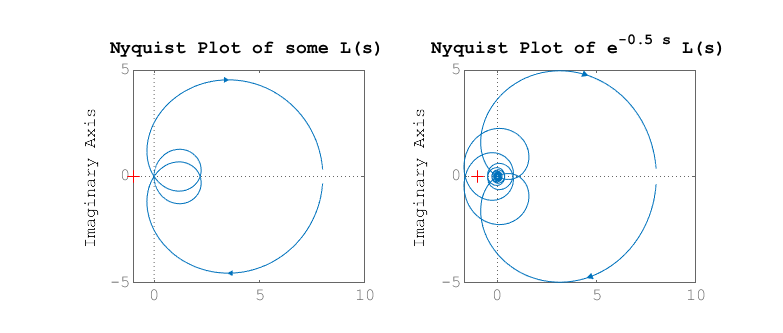
\includegraphics{Lab_5_Nyquist_Delay.eps}
  \caption[Nyquist Plot of Transfer Functions with and without a delay.]{Nyquist plots of an unknown loop transfer function \(L(s)\) (left) and of the same transfer function delayed by \SI{50}{\milli\second} (right).}
  \label{fig:lab5:delay}
\end{figure}
%
If you compare the Nyquist plot of \(L(s)\) with the Nyquist plot of \(e^{-\tau s} L(s)\) you should observe some similarities;
in fact, a number of points on the latter Nyquist plot look like a rotated version of the former Nyquist plot.
This is depicted by Figure~\ref{fig:lab5:delay}.
This notion, if put formally\footnote{If you do not see why, do not be alarmed. This lab will directly translate the specification for you.}, allows us to translate the earlier delay specification into the following phase margin specification: 
\begin{quote}
  The loop transfer function \(L(s)\) has a phase margin strictly greater than \(\tau \omega_{\mathrm{gc}}\) where \(\omega_{\mathrm{gc}}\) is the gain crossover frequency in \SI{}{\radian} and \(\tau\) is the delay in the loop in \SI{}{\second}.
\end{quote}
This is the primary specification you will meet in this lab to accomodate the delay.
Note that this specification only makes sense when \(L(s)\) is already stable in closed loop.

In practice, attempting to change the phase margin can also result in a changed gain crossover and thereby change what delays \(L(s)\) can afford.
The lag compensator in particular changes the gain crossover in order to increase the phase margin.
The lead compensator often results in a slightly higher gain crossover frequency.

\subsection{Part I: Delays and Stability}
Consider the simple proportional feedback loop
%
\begin{center}
  \begin{tikzpicture}[x=1in, y=1in]

    \node [draw, smooth_block] (Plant) {\(P(s)\)};
    \node [draw, smooth_block, left = 0.50 of Plant] (Gain1) {\(K\)};
    \node [draw, smooth_sum, left = 0.50 of Gain1] (Sum1) {};
    \node [right = 0.50 of Plant] (after_plant) {};
    \node [right = 0.50 of after_plant] (y) {};
    \node [left = 0.50 of Sum1] (r) {};

    \node [smooth_annotate, below = 0 of Gain1] {Controller};
    \node [smooth_annotate, below = 0 of Plant] {Plant};

    \draw [arrow, smooth_path]
      (Plant.east) -- (after_plant.base) -- (y.base) node [below right] {\(y\)};
    \draw [arrow, smooth_path]
      (Plant.east)
      --
      (after_plant.base)
      --
      +(0, -0.75)
      -|
      (Sum1.south)
      node [below right] {\(-\)};
    \draw [arrow, smooth_path]
      (Sum1.east)
      node [above right] {\(e\)}
      --
      (Gain1.west);
    \draw [arrow, smooth_path]
      (Gain1.east)
      --
      (Plant.west);
    \draw [arrow, smooth_path]
      (r.base)
      node [below left] {\(r\)}
      --
      (Sum1.west);
  \end{tikzpicture}
\end{center}
where \(P(s)\) is the dynamics of line-following drone.
Your first task is to
%
\begin{deliverable}[label={del:lab5:p1:1}]
  \textbf{Choose} a loop gain \(0 < K < 400\) so that the steady-state step tracking error is less than or equal to \(1\%.\)
\end{deliverable}
%
You will then acquire a Nyquist plot to verify stability of the closed loop system when there are no delays as well as acquire a Nyquist plot to demonstrate instability when the delay is introduced.
%
\begin{deliverable}[label={del:lab5:p1:2}]
  \textbf{Acquire} two Nyquist plots (using the Model Linearizer app) so that
  \begin{itemize}
    \item{one demonstrates the stability of the gain-compensated closed loop system when there is no delay and}
    \item{the other demonstrates the instability of the gain-compensated closed loop system with a delay.}
  \end{itemize}
\end{deliverable}
%
Finally, you will need to acquire a Bode plot of the undelayed open loop system in order to perform the Lead and Lag design procedures.
%
\begin{deliverable}[label={del:lab5:p1:3}]
  \textbf{Acquire} a Bode plot (using the Model Linearizer app) of the undelayed open loop system.
  \textbf{Place} a cursor at the gain crossover frequency on the magnitude plot.
\end{deliverable}
%
To complete these tasks, follow the next procedure.
%
\begin{procedure}[label={proc:lab5:1}]
  In this procedure you will determine a gain \(K\) and acquire the required Nyquist plots.
  You will also get a chance to simulate the system.
  \begin{enumerate}[label={(\arabic*)}]
    \item{%
      Assume the plant \(P(s)\) has a DC gain \(1.\)
      The transfer function from \(r(t)\) to \(e(t)\) is
      \[
        \frac{1}{1 + K P(s)}.
      \]
      \textbf{Choose} a gain \(K\) so that the DC gain of this transfer function is less than \(0.01.\)
      This assures a steady-state tracking error of less than \(1\%.\)
    }
    \item{%
      \textbf{Change} the variable \texttt{K} \emph{in the MATLAB script} ``procedure\_5\_1.m'' to match your chosen gain.
      \textbf{Run} the script.
    }
    \item{%
      \textbf{Open} the ``Lab\_5\_Model\_System.slx'' Simulink model and \textbf{ensure} that the switch is pointed towards the path without the ``Delay.''
    }
    \item{%
      The model should already be correctly configured with the ``Open Loop Input'' set to the signal \(e(t)\) and the ``Open Loop Output'' set to signal \(y(t).\)
      \textbf{Verify} this.
    }
    \item{%
      \textbf{Open} the Model Linearizer App and \textbf{acquire} a Nyquist plot.
      This produces part of Deliverable~\ref{del:lab5:p1:2}.
      Assuming \(P(s)\) has no unstable poles, \textbf{verify} that you have closed loop stability.
    }
    \item{%
      \textbf{Open} the Model Linearizer App and \textbf{acquire} a Bode plot.
      \textbf{Identify} the \SI{0}{\decibel} gain crossover and the phase margin.
      \textbf{Place} a cursor on the gain crossover frequency on the magnitude plot.
      This completes Deliverable~\ref{del:lab5:p1:3}.
    }
    \item{%
      If you are curious, \textbf{run} ``procedure\_5\_1\_simulate.m'' to see how the closed loop system behaves without a delay.
    }
    \item{%
      \textbf{Open} the ``Lab\_5\_Model\_System.slx'' Simulink model and \textbf{ensure} that the switch is pointed towards the path \textbf{with} the ``Delay.''
    }
    \item{%
      \textbf{Open} the Model Linearizer App and \textbf{acquire} a Nyquist plot.
      This completes Deliverable~\ref{del:lab5:p1:2}.
      Assuming \(P(s)\) has no unstable poles, \textbf{verify} that you do not have closed loop stability.
    }
    \item{%
      If you are curious, \textbf{run} ``procedure\_5\_1\_simulate.m'' to see how the closed loop system behaves with the delay.
      Expect the system to behave undesireably;
      It is even possible that the simulation stops early if the drone travels backwards!
    }
  \end{enumerate}
\end{procedure}

\subsection{Part II: Design a Lag controller}
One way to increase the phase margin of a loop transfer function is to introduce a Lag controller.
Lag controllers decrease the gain so as to change the gain crossover;
changing the gain crossover in turn changes the phase margin.
In this part the closed loop system takes the form
%
\begin{center}
  \begin{tikzpicture}[x=1in, y=1in]

    \node [draw, smooth_block] (Plant) {\(K P(s)\)};
    \node [draw, smooth_block, left = 0.50 of Plant] (Gain1) {\(C_\mathrm{lag}(s)\)};
    \node [draw, smooth_sum, left = 0.50 of Gain1] (Sum1) {};
    \node [right = 0.50 of Plant] (after_plant) {};
    \node [right = 0.50 of after_plant] (y) {};
    \node [left = 0.50 of Sum1] (r) {};

    \node [smooth_annotate, below = 0 of Gain1] {Controller};
    \node [smooth_annotate, below = 0 of Plant] {Plant};

    \draw [arrow, smooth_path]
      (Plant.east) -- (after_plant.base) -- (y.base) node [below right] {\(y\)};
    \draw [arrow, smooth_path]
      (Plant.east)
      --
      (after_plant.base)
      --
      +(0, -0.75)
      -|
      (Sum1.south)
      node [below right] {\(-\)};
    \draw [arrow, smooth_path]
      (Sum1.east)
      node [above right] {\(e\)}
      --
      (Gain1.west);
    \draw [arrow, smooth_path]
      (Gain1.east)
      --
      (Plant.west);
    \draw [arrow, smooth_path]
      (r.base)
      node [below left] {\(r\)}
      --
      (Sum1.west);
  \end{tikzpicture}
\end{center}
%
where
\[
  C_\mathrm{lag}(s)
    =
      \frac{\alpha T s + 1}{T s + 1}
  ,
  \;
  0 < \alpha < 1
  ,
  \;
  T > 0.
\]
is a Lag compensator with \SI{0}{\decibel} DC gain.
Your task is to find \(\alpha\) and \(T\) in terms of a phase margin specification and the Bode plot of \(K P(s)\) --- determined by Deliverable~\ref{del:lab5:p1:3} --- to complete the Lag control design.
%
\begin{deliverable}[label={del:lab5:p2:1}]
  Let \(\omega_\mathrm{gc}\) determine the \SI{0}{\decibel} gain crossover frequency (in \SI{}{\radian}) of \(K P(s).\) 
  This can determined by looking at the Bode plot from Deliverable~\ref{del:lab5:p1:3}.
  \textbf{Design} a Lag compensator (determine \(\alpha\) and \(T\)) so that the Bode plot of the compensated open loop system has a phase margin strictly greater than \(\frac{6\omega_\mathrm{gc}}{100}~\mathrm{rad}.\)
  \textbf{You must show the use of the design equations for full marks.}
\end{deliverable}
%
You will then acquire a Nyquist plot to demonstrate that the delayed system has been stabilized with the Lag compensator.
%
\begin{deliverable}[label={del:lab5:p2:2}]
  \textbf{Acquire} a Nyquist plot demonstrating the Lag compensated system \emph{with delay} is closed loop stable.
\end{deliverable}
%
\begin{procedure}[label={proc:lab5:2}]
  In this procedure you will design a Lag compensator, using the content you learned in your course, and simulate the delayed closed loop system.
  \begin{enumerate}[label={(\arabic*)}]
    \item{%
      Using the \SI{0}{\decibel} gain crossover frequency \(\omega_\mathrm{gc}\) found for \(K P(s)\) in Deliverable~\ref{del:lab5:p1:3} the engineers at VenX have determined that compensated closed loop system must have a phase margin strictly greater than
      \[
        \frac{6\omega_\mathrm{gc}}{100}~\mathrm{rad}.
      \]
      Using the Bode plot in Deliverable~\ref{del:lab5:p1:3}, \textbf{determine} the required gain crossover to achieve this specification.
    }
    \item{%
      \textbf{Choose} \(\alpha\) and \(T\) in a way to meet this specification.
      This produces Deliverable~\ref{del:lab5:p2:1}.
    }
    \item{%
      \textbf{Change} the variable \texttt{alpha} and \texttt{T} \emph{in the MATLAB script} ``procedure\_5\_2.m'' to match your chosen parameters.
      \textbf{Run} the script.
    }
    \item{%
      \textbf{Open} the ``Lab\_5\_Model\_System.slx'' Simulink model and \textbf{ensure} that the switch is pointed towards the path \textbf{with} the ``Delay.''
    }
    \item{%
      \textbf{Open} the Model Linearizer App and \textbf{acquire} a Nyquist plot.
      This completes Deliverable~\ref{del:lab5:p2:2}.
      Assuming \(P(s)\) has no unstable poles, \textbf{verify} that you do not have closed loop stability.
    }
  \end{enumerate}
\end{procedure}

\subsection{Part III: Design a Lead controller}
Another way to increase the phase margin of a loop transfer function is to introduce a Lead controller.
Lead controllers add phase at the crossover frequency.
In this part the closed loop system takes the form
%
\begin{center}
  \begin{tikzpicture}[x=1in, y=1in]

    \node [draw, smooth_block] (Plant) {\(K P(s)\)};
    \node [draw, smooth_block, left = 0.50 of Plant] (Gain1) {\(C_\mathrm{lead}(s)\)};
    \node [draw, smooth_sum, left = 0.50 of Gain1] (Sum1) {};
    \node [right = 0.50 of Plant] (after_plant) {};
    \node [right = 0.50 of after_plant] (y) {};
    \node [left = 0.50 of Sum1] (r) {};

    \node [smooth_annotate, below = 0 of Gain1] {Controller};
    \node [smooth_annotate, below = 0 of Plant] {Plant};

    \draw [arrow, smooth_path]
      (Plant.east) -- (after_plant.base) -- (y.base) node [below right] {\(y\)};
    \draw [arrow, smooth_path]
      (Plant.east)
      --
      (after_plant.base)
      --
      +(0, -0.75)
      -|
      (Sum1.south)
      node [below right] {\(-\)};
    \draw [arrow, smooth_path]
      (Sum1.east)
      node [above right] {\(e\)}
      --
      (Gain1.west);
    \draw [arrow, smooth_path]
      (Gain1.east)
      --
      (Plant.west);
    \draw [arrow, smooth_path]
      (r.base)
      node [below left] {\(r\)}
      --
      (Sum1.west);
  \end{tikzpicture}
\end{center}
%
where
\[
  C_\mathrm{lead}(s)
    =
      \frac{\alpha T s + 1}{T s + 1}
  ,
  \;
  \alpha > 1
  ,
  \;
  T > 0.
\]
is a Lead compensator with unit DC gain.
Your task is to find \(\alpha\) and \(T\) in terms of a phase margin specification and the Bode plot of \(K P(s)\) --- determined by Deliverable~\ref{del:lab5:p1:3} --- to complete the Lead control design.
%
\begin{deliverable}[label={del:lab5:p3:1}]
  Let \(\omega_\mathrm{gc}\) determine the \SI{0}{\decibel} gain crossover frequency (in \SI{}{\radian}) of \(K P(s).\) 
  This can determined by looking at the Bode plot from Deliverable~\ref{del:lab5:p1:3}.
  \textbf{Design} a Lead compensator (determine \(\alpha\) and \(T\)) so that the Bode plot of the compensated open loop system has a phase margin strictly greater than \(\frac{6\omega_\mathrm{gc}}{100}~\mathrm{rad}.\)
  \textbf{You must show the use of the design equations for full marks.}
\end{deliverable}
%
You will then acquire a Nyquist plot to demonstrate that the delayed system has been stabilized with the Lead compensator.
%
\begin{deliverable}[label={del:lab5:p3:2}]
  \textbf{Acquire} a Nyquist plot demonstrating the Lead compensated system \emph{with delay} is closed loop stable.
\end{deliverable}
%
\begin{procedure}[label={proc:lab5:3}]
  In this procedure you will design a Lead compensator, using the content you learned in your course, and simulate the delayed closed loop system.
  \begin{enumerate}[label={(\arabic*)}]
    \item{%
      Using the \SI{0}{\decibel} gain crossover frequency \(\omega_\mathrm{gc}\) found for \(K P(s)\) in Deliverable~\ref{del:lab5:p1:3} the engineers at VenX have determined that compensated closed loop system must have a phase margin strictly greater than
      \[
        \frac{6\omega_\mathrm{gc}}{100}~\mathrm{rad}.
      \]
      Using the Bode plot in Deliverable~\ref{del:lab5:p1:3}, \textbf{determine} the required phase addition to meet this specification.
    }
    \item{%
      \textbf{Choose} \(\alpha\) and \(T\) in a way to meet this specification.
      This produces Deliverable~\ref{del:lab5:p3:1}.
    }
    \item{%
      \textbf{Change} the variable \texttt{alpha} and \texttt{T} \emph{in the MATLAB script} ``procedure\_5\_3.m'' to match your chosen parameters.
      \textbf{Change} the gain \texttt{K} in that same script if your design procedure demands it.
      \textbf{Run} the script.
    }
    \item{%
      \textbf{Open} the ``Lab\_5\_Model\_System.slx'' Simulink model and \textbf{ensure} that the switch is pointed towards the path \textbf{with} the ``Delay.''
    }
    \item{%
      \textbf{Open} the Model Linearizer App and \textbf{acquire} a Nyquist plot.
      This completes Deliverable~\ref{del:lab5:p3:2}.
      Assuming \(P(s)\) has no unstable poles, \textbf{verify} that you do not have closed loop stability.
    }
  \end{enumerate}
\end{procedure}

\subsection{Part IV: Simulating the Real System}
In Parts II and III you designed and verified Lag and Lead compensators that ensure closed loop stability of a plant with delay.
This was verified using the Nyquist plots of Deliverable~\ref{del:lab5:p2:2} and~\ref{del:lab5:p3:2}.
In this part, you will simulate the real closed loop system with delays.
The true closed loop system takes the form
%
\begin{center}
  \begin{tikzpicture}[x=1in, y=1in]

    \node [draw, smooth_block] (Plant) {\(P(s)\)};
    \node [draw, smooth_block, left = 0.40 of Plant] (delay1) {%
      \(e^{-\frac{\tau}{2} s}\)
    };
    \node [draw, smooth_block, right = 0.40 of Plant] (delay2) {%
      \(e^{-\frac{\tau}{2} s}\)
    };
    \node [draw, smooth_block, left = 0.40 of delay1] (Gain1) {%
      \(K\frac{\alpha T s + 1}{T s + 1}\)%
    };
    \node [draw, smooth_sum, left = 0.40 of Gain1] (Sum1) {};
    \node [right = 0.40 of delay2] (after_plant) {};
    \node [right = 0.40 of after_plant] (y) {};
    \node [left = 0.40 of Sum1] (r) {};

    \node [smooth_annotate, below = 0 of Gain1] {Controller};
    \node [smooth_annotate, below = 0 of Plant] {Plant};
    \node [smooth_annotate, below = 0 of delay1] {Send Delay};
    \node [smooth_annotate, below = 0 of delay2] {Receive Delay};

    \draw [arrow, smooth_path]
      (Plant.east)
      --
      (delay2.west);
    \draw [arrow, smooth_path]
      (delay2.east) -- (after_plant.base) -- (y.base) node [below right] {\(y\)};
    \draw [arrow, smooth_path]
      (delay2.east)
      --
      (after_plant.base)
      --
      +(0, -0.75)
      -|
      (Sum1.south)
      node [below right] {\(-\)};
    \draw [arrow, smooth_path]
      (Sum1.east)
      node [above right] {\(e\)}
      --
      (Gain1.west);
    \draw [arrow, smooth_path]
      (Gain1.east)
      --
      (delay1.west);
    \draw [arrow, smooth_path]
      (delay1.east)
      --
      (Plant.west);
    \draw [arrow, smooth_path]
      (r.base)
      node [below left] {\(r\)}
      --
      (Sum1.west);
  \end{tikzpicture}
\end{center}
%
The ``Send Delay'' captures the amount of time the plant has to wait to see an update from the controller on the ground while the ``Receive Delay'' captures the amount of time the controller has to wait to see an updated output.
From a networking perspective, this is lower bounded by the ping time\footnote{since it ignores any computational delays.}.
If you designed your Lag and Lead compensators correctly in Parts II and III, then you should expect them to perform adequately.
Remember, stability is the primary characteristic of concern in this discussion.
Do not be alarmed if the settling time or overshoot is undesireable.

There are precisely two deliverables for this part.
First you will simulate the real system against the Lag compensator to produce
%
\begin{deliverable}[label={del:lab5:p4:1}]
  \textbf{Acquire} Figure 542 generated by ``procedure\_5\_4\_simulate.m.''
\end{deliverable}
%
Second, you will simulate the real system against the Lead compensator to produce
%
\begin{deliverable}[label={del:lab5:p4:2}]
  \textbf{Acquire} Figure 552 generated by ``procedure\_5\_5\_simulate.m.''
\end{deliverable}
%
To do so, follow the next couple procedures.
%
\begin{procedure}[label={proc:lab5:4}]
  In this procedure you will simulate the real closed loop system with your Lag compensator.
  \begin{enumerate}[label={(\arabic*)}]
    \item{%
      \textbf{Run} ``procedure\_5\_4\_simulate.m.''
    }
    \item{%
      \textbf{Save} Figure 542.
      \textbf{Verify} the simulatation ran to completion (\SI{240}{\second}) and that the error settles.
      If there are oscillations, they should decay.
      This produces Deliverable~\ref{del:lab5:p4:1}.
    }
  \end{enumerate}
\end{procedure}
%
\begin{procedure}[label={proc:lab5:5}]
  In this procedure you will simulate the real closed loop system with your Lead compensator.
  \begin{enumerate}[label={(\arabic*)}]
    \item{%
      \textbf{Run} ``procedure\_5\_5\_simulate.m.''
    }
    \item{%
      \textbf{Save} Figure 552.
      \textbf{Verify} the simulatation ran to completion (\SI{240}{\second}) and that the error settles.
      If there are oscillations, they should decay.
      This produces Deliverable~\ref{del:lab5:p4:2}.
    }
  \end{enumerate}
\end{procedure}


\section{Report Deliverable}\label{Lab:5:Report}
You are almost done the lab component of this course!
As usual, you are expected to submit a report demonstrating that you completed the lab and that you understand the tasks performed.
In addition to including
\begin{itemize}
  \item{Deliverable~\ref{del:lab5:p1:1},}
  \item{Deliverable~\ref{del:lab5:p1:2},}
  \item{Deliverable~\ref{del:lab5:p1:3},}
  \item{Deliverable~\ref{del:lab5:p2:1},}
  \item{Deliverable~\ref{del:lab5:p2:2},}
  \item{Deliverable~\ref{del:lab5:p3:1},}
  \item{Deliverable~\ref{del:lab5:p3:2},}
  \item{Deliverable~\ref{del:lab5:p4:1},}
  \item{Deliverable~\ref{del:lab5:p4:2},}
\end{itemize}
in your report, you are required to answer the questions of the following deliverable.
Make sure to leverage your other deliverables in your answers!
\begin{deliverable}[label={lab5:report}]
  \begin{enumerate}[label={(\arabic*)}]
    \item{%
      In both the Lead and Lag design procedures you had to add more phase (or decrease the gain crossover more) than what the phase margin specification demands.
      Acquire a Bode plot of your Lead and Lag compensators to \textbf{explain why}.
      \label{lab5:report:q1}
    }
    \item{%
      \textbf{Describe} the qualitative differences between the final closed loop response of your Lag compensated and Lead compensated systems.
      Touch on characteristics like
      \begin{itemize}
        \item{
          the overshoot,
        }
        \item{
          the settling time and
        }
        \item{
          the time to peak.
        }
      \end{itemize}
      Use the simulations in Deliverables~\ref{del:lab5:p4:1} and~\ref{del:lab5:p4:2} in your discussion.
      \label{lab5:report:q2}
    }
    \item{%
      \textbf{Describe} how you would choose between a Lead compensator or Lag compensator.

      Ensure to leverage the Nyquist plots in Deliverables~\ref{del:lab5:p2:2} and~\ref{del:lab5:p3:2} as well as your answers to~\ref{lab5:report:q1} and~\ref{lab5:report:q2} in your discussion.

      \label{lab5:report:q3}
    }
    \item{%
      Using the original phase margin \(\phi\) and gain crossover \(\omega_\mathrm{gc}\) of \(K P(s)\) --- both of which can be found by looking at the Bode plot of Deliverable~\ref{del:lab5:p1:3} --- \textbf{compute} the maximum delay
      \[
        \tau_\mathrm{max} = \frac{\phi}{\omega_\mathrm{gc}}
      \]
      the uncompensated system could afford before becoming unstable.
      \label{lab5:report:q4}
    }
    \item{%
      A local WiFi network usually sees a round trip time for network packets of around \SI{1}{\milli\second} to \SI{3}{\milli\second}.

      \textbf{Would} your uncompensated system be stable if the feedback loop involved communication over a similar wireless network with comparable delays?
      If not, would the compensated system be stable?
      \label{lab5:report:q5}
    }
    \item{%
      The delay in the real system of Part IV was a total of \SI{60}{\milli\second}:
      there was a send delay of \SI{30}{\milli\second} and a receive delay of \SI{30}{\milli\second}.

      In 4G/LTE communication networks the mean round trip time of a packet is around \SI{50}{\milli\second}.

      \textbf{Would} your uncompensated system be stable if the feedback loop involved communication over a similar wireless network with comparable delays?
      If not, would the compensated system be stable?
      \label{lab5:report:q6}
    }
    \item{%
      Using the Nyquist plot of the \emph{delayed} system acquired in Deliverable~\ref{del:lab5:p1:2}, \textbf{determine} if there exists an additional proportional feedback gain \(\hat{K} \in \mathbb{R}\) that would stabilize the system \(K P(s)\) even in the presence of the \SI{60}{\milli\second} delay.

      To be clear: Can you find a (positive or negative) gain \(\hat{K}\) that renders the closed loop system
      %
      \begin{center}
        \begin{tikzpicture}[x=1in, y=1in]

          \node [draw, smooth_block] (Plant) {\(K P(s)\)};
          \node [draw, smooth_block, right = 0.4 of Plant] (Delay) {%
            \(e^{-0.06 s}\)
          };
          \node [draw, smooth_block, left = 0.40 of Plant] (Gain1) {%
            \(\hat{K}\)%
          };
          \node [draw, smooth_sum, left = 0.40 of Gain1] (Sum1) {};
          \node [right = 0.40 of Delay] (after_plant) {};
          \node [right = 0.40 of after_plant] (y) {};
          \node [left = 0.40 of Sum1] (r) {};

          \draw [arrow, smooth_path]
            (Plant.east)
            --
            (Delay.west);
          \draw [arrow, smooth_path]
            (Delay.east) -- (after_plant.base) -- (y.base) node [below right] {\(y\)};
          \draw [arrow, smooth_path]
            (Delay.east)
            --
            (after_plant.base)
            --
            +(0, -0.60)
            -|
            (Sum1.south)
            node [below right] {\(-\)};
          \draw [arrow, smooth_path]
            (Sum1.east)
            node [above right] {\(e\)}
            --
            (Gain1.west);
          \draw [arrow, smooth_path]
            (Gain1.east)
            --
            (Plant.west);
          \draw [arrow, smooth_path]
            (r.base)
            node [below left] {\(r\)}
            --
            (Sum1.west);
        \end{tikzpicture}
      \end{center}
      %
      stable?

      If it exists, does this closed loop system have a larger or smaller steady-state error in comparison to the undelayed \(K P(s).\)

      What does this suggest about the effect of delays on performance?
      \label{lab5:report:q7}
    }
  \end{enumerate}
\end{deliverable}

\subsection{Grading Scheme}
The grading scheme is shown in Table~\ref{tab:lab5:grading}. The breakdown of
your grade is shown per deliverable except in the case of the lab
questions where it is shown per question.
%
\begin{table}
\centering
\begin{tabular}{c|l|c}
        & Deliverable           & Marks  \\ \hline
        & \ref{del:lab5:p1:1}         & 4       \\ \hline
        & \ref{del:lab5:p1:2}         & 4       \\ \hline
        & \ref{del:lab5:p1:3}         & 4      \\ \hline
        & \ref{del:lab5:p2:1}         & 4      \\ \hline
        & \ref{del:lab5:p2:2}         & 4       \\ \hline
        & \ref{del:lab5:p3:1}         & 4       \\ \hline
        & \ref{del:lab5:p3:2}         & 4       \\ \hline
        & \ref{del:lab5:p4:1}         & 4       \\ \hline
        & \ref{del:lab5:p4:2}         & 4       \\ \hhline{=|=|=}
Lab Subtotal&                       & 36      \\ \hhline{=|=|=}
        & \ref{lab5:report}~\ref{lab5:report:q1}  & 2       \\ \hline
        & \ref{lab5:report}~\ref{lab5:report:q2}  & 2       \\ \hline
        & \ref{lab5:report}~\ref{lab5:report:q3}  & 2       \\ \hline
        & \ref{lab5:report}~\ref{lab5:report:q4}  & 2      \\ \hline
        & \ref{lab5:report}~\ref{lab5:report:q5}  & 2      \\ \hline
        & \ref{lab5:report}~\ref{lab5:report:q6}  & 2      \\ \hline
        & \ref{lab5:report}~\ref{lab5:report:q7}  & 2      \\ \hhline{=|=|=}
Report Subtotal&  & 14 \\ \hhline{=|=|=}
  Total &                       & 50
\end{tabular}
\caption[Grading Scheme for Lab 5]{Grading scheme for Lab 5.}
\label{tab:lab5:grading}
\end{table}
%
